\documentclass{tudelft-report}
\usepackage{acronym}
\usepackage{lscape}
\usepackage{gensymb}
\usepackage{textcomp}
\usepackage{multicol}
\usepackage[version=3]{mhchem} % Package for chemical equation typesetting
\usepackage{siunitx} % Provides the \SI{}{} and \si{} command for typesetting SI units
\usepackage{graphicx} % Required for the inclusion of images
\usepackage{natbib} % Required to change bibliography style to APA
\usepackage{amsmath} % Required for some math elements 
%\usepackage[colorlinks=true,linkcolor=blue]{hyperref}
\usepackage{parskip}
\usepackage[nameinlink]{cleveref}
\usepackage[]{caption}

\usepackage{todonotes}
\linespread{1.15}
\newcommand{\todoref}[1]{\todo[backgroundcolor=blue!20!white]{#1}}
\newcommand{\comm}[1]{\todo[backgroundcolor=green!20!white]{#1}}
\setlength{\marginparwidth}{2cm}
\usepackage{titlesec}
\usepackage{sectsty}


\titleformat*{\subsubsection}{\bfseries}

\titleformat*{\paragraph}{\bfseries}
\begin{document}

%% Use Roman numerals for the page numbers of the title pages and table of
%% contents.
\frontmatter

\title[Applied in Autonomous Drone Racing]{Efficient Detection of Wire Frame Objects on Micro-Air Vehicles}
\author{P.\ Duernay}
\affiliation{Delft University of Technology}
%\coverimage{cover.jpg}
%\makecover

%% Include an optional title page.
\begin{titlepage}
	
	\begin{center}
		
		%% Insert the TU Delft logo at the bottom of the page.
		\begin{tikzpicture}[remember picture,overlay]
		\node at (current page.south)[anchor=south,inner sep=0pt]{
			
\includegraphics{cover/logo}
		};
		\end{tikzpicture}
		
		%% Extra whitespace at the top.
		\vspace*{2\bigskipamount}
		
		%% Print the title in cyan.
		{\makeatletter
			\titlestyle\color{tudelft-cyan}\Huge\@title
			\makeatother}
		
		%% Print the optional subtitle in black.
		{\makeatletter
			\ifx\@subtitle\undefined\else
			\bigskip
			\titlefont\titleshape\LARGE\@subtitle
			\fi
			\makeatother}
		
		\bigskip
		\bigskip
		
		by
		%door
		
		\bigskip
		\bigskip
		
		%% Print the name of the author.
		{\makeatletter
			\titlefont\Large\bfseries\@author
			\makeatother}
		
		\vfill
		
		in partial fulfillment of the requirements for the degree of
		%in overeenstemming met de vereisten voor het verkrijgen van de graad van
		
		\bigskip
		\bigskip
		
		{\bfseries Master of Science}
		
		in Embedded Systems
		
		\bigskip
		\bigskip
		
		at the Delft University of Technology,
		%aan de Technische Universiteit Delft,
		
		to be defended publicly on Tuesday January 1, 2013 at 10:00 AM.
		%in het openbaar de verdedigen op dinsdag 1 januari om 10:00 uur.
		
		\vfill
		
		\begin{tabular}{lll}
			%% Add additional information here, per faculty requirements, e.g
			%    Student number: & 1234567 \\
			%    Project duration: & \multicolumn{2}{l}{March 1, 2012 -- January 1, 2013} \\
			Supervisor: & Prof.\ dr.\ ir.\ D. M. J\ Tax \\
			Thesis committee:
			& Prof.\ dr.\ C.\ F.\ Guido de Croon, & TU Delft \\
			& Dr.\ E.\ L.\ Brown, & TU Delft \\
			& Ir.\ M.\ Scott, & Acme Corporation
		\end{tabular}
		
		%% Only include the following lines if confidentiality is applicable.
		\bigskip
		\bigskip
		\emph{This thesis is confidential and cannot be made public until December 31, 2013.}
		%\emph{Op dit verslag is geheimhouding van toepassing tot en met 31 december 2013.}
		
		\bigskip
		\bigskip
		An electronic version of this thesis is available at \url{http://repository.tudelft.nl/}.
		%Een elektronische versie van dit verslag is beschikbaar op \url{http://repository.tudelft.nl/}.
		
	\end{center}
	
\end{titlepage}



\chapter*{Preface}
\setheader{Preface}

Preface\ldots


\begin{flushright}
	{\makeatletter\itshape
		\@author \\
		Delft, January 2013
		\makeatother}
\end{flushright}



\tableofcontents

%% Use Arabic numerals for the page numbers of the chapters.
\mainmatter

\chapter*{Summary}
\addcontentsline{toc}{chapter}{Summary}
\setheader{Summary}

\ac{MAV} are an emerging technology that supports a wide range of applications. Thereby the robust estimation of an \ac{MAV}'s state within its environment is crucial to ensure safe operation. In  indoor scenarios cameras are one of the predominant choices for state estimation sensors. This requires Computer Vision algorithms to interpret the obtained high dimensional signal. An application that allows the competitive evaluation of control and state estimation algorithms is \ac{MAV} Racing such as the \ac{IROS}2018 Autonomous Drone Race. Thereby a race court consisting of several race gates has to be followed. For a fast flight during such a race court the detection of the racing gates with a camera can be used in a high level control loop. As these object consist only of small structures that are spread across large parts of the image, this gives rise to a challenging Object Detection problem.

In recent years \acp{CNN} showed promising results on various vision tasks. However, due to their computational complexity the deployment on mobile devices remains a challenge. Furthermore, \acp{CNN} typically require a vast amount of training data. This work defines the class of \acp{EWFO} and studies their detection on \acp{MAV} with \ac{Yolo}V3. For the training, data is generated with a graphical engine. 

The experiments conducted in simulation show how \acp{EWFO} are harder to detect than filled objects as the detector can be confused to patterns present in the empty part. Particularly for larger objects the detection performance decreases. We give several recommendations how to generate data for the detection of \acp{EWFO} on \acp{MAV}. These include how to include variations in background as well as the camera placement. Finally, we study the incorporation of image augmentation techniques to transfer the detector to the real world. We can report that especially modelling lens distortion improves the performance on the real data. Nevertheless, a reality gap remains that can not fully be explained.

Furthermore, different architectures are studied for the detection of \acp{EWFO}. It can be seen how a relatively shallow network of 9 layers can be used for the detection of \acp{EWFO} on \acp{MAV}. A further reduction in weights leads to a gradual decrease in performance. 

Based on the gained insights the deployment of a detector on an example system is studied. A detection performance/speed trade-off is evaluated. The final detector achieves 32\% $ap_{60}$ at a frame rate of 12 Hz on a real world test set created during this work.



\chapter*{Glossary}
\begin{acronym}
	\acro{IR}{Infrared}
	\acro{LIDAR}{Light Detection And Ranging}
	\acro{EWFO}{Empty Wire Frame Objects}
	\acro{FoV}{Field of View}
	\acro{CNN}{Convolutional Neural Network}
	\acro{GPS}{Global Positioning System}
	\acro{GPU}{Graphical Processing Unit}
	\acro{MAV}{Micro-Air Vehicle}
	\acro{DR}{Domain Randomization}
	\acro{TO}{Target Object}
	\acro{DSC}{Depthwise Separable Convolution}
	\acro{IMU}{Inertial Measurement Unit}
	\acrodefplural{IMU}[IMUs]{Inertial Measurement Units}
	\acro{FPV}{First Person View}
	\acro{IROS}{International Conference of Intelligent Robots}
	\acro{i.i.d.}{independently identically distributed}
\end{acronym}
\chapter{Introduction}
\label{sec:intro}
\acresetall
\acp{MAV} such as a Quadrotor-\ac{MAV} displayed in \autoref{fig:mav} are an emerging technology that supports society in a wide range of consumer, industrial and safety applications. For example \acp{MAV} are used to deliver medicine \cite{Shankland2018}, fight fires \cite{KateBaggaley2017} or even find survivors in disaster situations \cite{JoshuaBateman2017}.

\begin{figure}[b]
	\centering
	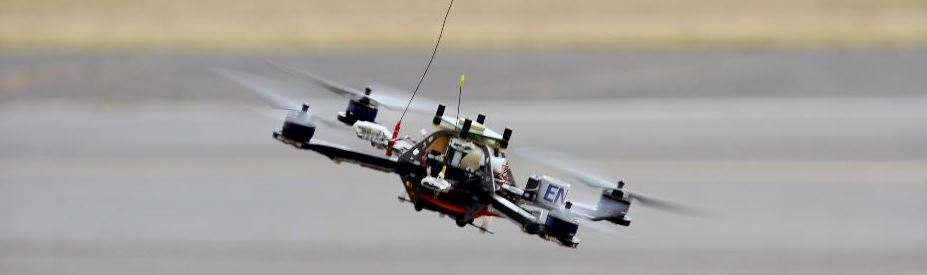
\includegraphics[width=\textwidth]{fig/mav}
	\caption{An example of a Quadrotor-\ac{MAV}-Platform that is used in this thesis.}
	\label{fig:mav}
\end{figure}

Especially in emergency scenarios the fast and safe flight of \acp{MAV} is crucial to deliver help quickly and save human lives. However, due to the complexity of such missions as well as the difficulty to control an \ac{MAV} in disaster scenarios, often multiple human operators are required in order to ensure safe operation \cite{Murphy2016}. With humans in the loop a constant connection between the \ac{MAV} and the operators is required which not only uses energy and requires infrastructure but also significantly increases the reaction time. Enabling \acp{MAV} to fly more autonomously could allow human operators to control more \acp{MAV} and thus to improve the support in emergency situations.

A major challenge on the way to the full autonomous flight of \acp{MAV} is the accurate estimation of the \ac{MAV}'s state within its environment. The system is highly dynamic so position and orientation can change rapidly. At the same time noise introduced by motor vibrations makes the position estimation with only on-board \acp{IMU} too inaccurate \cite{Mohamed2014}. \ac{LIDAR}-sensors can capture long and wide range 3D information but the sensors are typically heavy and require a significant amount of energy. \ac{IR} sensors can cover distance information but are often limited in their \ac{FoV} as well as in their range. External infrastructure like \ac{GPS} and optical tracking systems can provide accurate measurements but there is no guarantee that such systems are present in real world applications. Cameras on the other hand are cheap, lightweight and can measure long range distance information. This makes them a suitable choice as a sensor for on-board state estimation on light \acp{MAV} \cite{Elbanhawi2017}.

However, the signal delivered by the camera is high dimensional and can not directly be interpreted as position or orientation measurements. Computer Vision algorithms are required to interpret the image and extract relevant information. This can be done by designing an algorithm manually or learning the image processing from annotated examples. In particular Deep Learning based methods aim to combine whole Computer Vision pipelines into one mapping that transforms the raw input image into a task dependent output. Experiments have shown how Deep Learning based methods outperform traditional Machine Learning approaches and manually crafted algorithms \cite{Razavian}. This made them the predominant choice for almost any vision task.

The hereby used \acp{CNN} are designed in a hierarchical way, using multiple layers that are evaluated sequentially. An example architecture is displayed in \Cref{fig:cnn_example}. The network transforms an image of size 224x224 from its input (left) to a task dependent output (right). In this case a classification network predicting 1000 class probabilities is displayed. Each layer applies a non-linear transformation for which the parameters are learned during training. By stacking more layers on top of each other (deepening) and increasing the number of nodes $D$ per layer (widening), highly non-linear functions can be modelled. 

Experiments have shown the superior performance of particularly deep/wide models \cite{He, He2015, Szegedy2014, Zagoruyko2016}. However, this model flexibility assumed to be the reason for their superior performance also leads to immense requirements in computational resources. For example a state-of-the-art Computer Vision model \cite{He2015} contains 60.2 million parameters and one inference requires 11.3 billion floating point operations \cite{Tschannen2017}. 

\begin{figure}[bhtp]
	\centering
	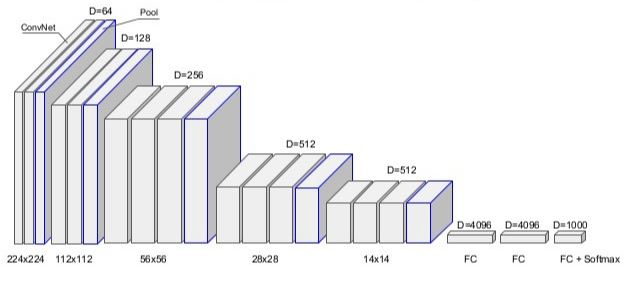
\includegraphics[width=0.8\textwidth]{fig/vgg_architecture}
	\caption{Example Architecture of a \ac{CNN}.}
	\label{fig:cnn_example}
\end{figure}

Robotic platforms like \acp{MAV} have limited resources in terms of processing power and battery life. Hence, the use of \acp{CNN} on such devices is still an open challenge. Research has addressed to reduce the number of computations in Deep Learning models on multiple levels\cite{YoungwanLee, Zagoruyko2016, Howard2017, Ghosh2017, Sandler2018, Zhang2017a}. However, the investigation of relatively shallow models with less than ten layers received only little attention by the research community.

This work investigates the deployment of a Deep Learning based Computer Vision pipeline on a \ac{MAV}. The method is applied in the challenging scenario of Autonomous Drone Racing at the \ac{IROS} 2018. Within the race court several metal gates are placed and need to be passed one after another. Detecting the gates allows to estimate the \ac{MAV}'s relative position and to calculate the flying trajectory. An overview of the race court and the racing gates at the \ac{IROS} 2016 Autonomous Drone Race can be seen in \Cref{fig:race_court}.

\begin{figure}[bhtp]
	\centering
	\begin{minipage}{0.45\linewidth}
	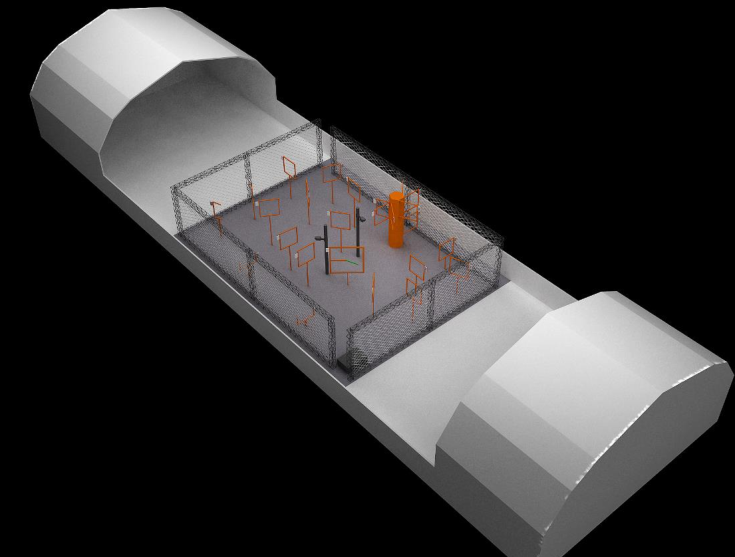
\includegraphics[width=\textwidth]{fig/race_court}
	\end{minipage}\hfill
\begin{minipage}{0.45\linewidth}
	\includegraphics[width=\textwidth]{fig/race_court_side}
\end{minipage}
\caption{Example Images of the \ac{IROS} 2016 Autonomous Drone Race}
\label{fig:race_court}
\end{figure}

The thesis builds on previous work by Ozo et. al \todoref{Reference to Current Method once it is published} which uses a manually crafted image processing method to detect the racing gates. Although fast to execute the method is very sensitive to illumination changes. Moreover, the algorithm fails when the objects are too far away or the frame is very thin. In order to develop a more robust method, this thesis investigates a learning based approach to the detection of racing gates.

Object Detection is one of the most intensively studied topics in Computer Vision. However, the objects investigated are usually solid and contain complex shapes. For example a pedestrian consist of body parts and a face. A box that surrounds the object mostly contains parts with distinctive shape an/or texture. A Computer Vision model can use these features for detection. The racing gates in contrast are of different nature. As can be seen in \Cref{fig:race_court} a box that surrounds the object would largely contain background. Hence, this part can not be used as a hint whether an object is present. Instead it can contain other objects even other gates that might distract a detector. Additionally, the object parts themselves are of very thin structure and can be hardly visible. Thus, a detector needs to make use of fine-grain structures, while ignoring the majority of the image. This introduces a particular vision task that even humans have a hard time at solving \footnote{The unconvinced reader can try to count the number of gates visible in the right image of \Cref{fig:race_court}} and that affects the training and design of a Computer Vision pipeline that aims to detect these kind of objects.

This thesis defines a class of objects as \textbf{\ac{EWFO}} studies methods for their detection. The definition is given as follows:

\paragraph{Definition - Empty Wire Frame Objects}	
\begin{enumerate}
	\item \textbf{Empty.} The object parts are sparse. The bounding box around the object is largely occupied by background.
	\item \textbf{Wire.} The object parts themselves are thin structures. The object does not consist of complex but only basic geometric shapes like corners, lines and edges.
	\item \textbf{Frame.} The object parts can be spread over large parts of the image, while the point of interest is in the center of this part.

\end{enumerate}

The detection of \ac{EWFO} is studied in the examples of the \ac{IROS} drone race gates. These can be seen can be seen in \Cref{fig:gates}. The image shows the \textit{Closed Gate} as well as the \textit{Jungle Gate}. Thereby the orange part is considered to be the object of interest. To the best of the authors knowledge \ac{EWFO} have not been particularly addressed in Computer Vision. In \cite{Falanga} and \cite{Li2018a} the authors also detect racing gates, however the used objects contain more structure than the ones investigated in this thesis. \citeauthor{Jung2018} present a framework to detect similar objects in \cite{Jung} and \cite{Jung2018} but do not study the particular effects of the object shape. This work particularly addresses the implications of the object shape in using a Deep Learning based detection system for \ac{EWFO}.

\begin{figure}[bhtp]
	\centering
	\begin{minipage}{0.45\linewidth}
		\centering
		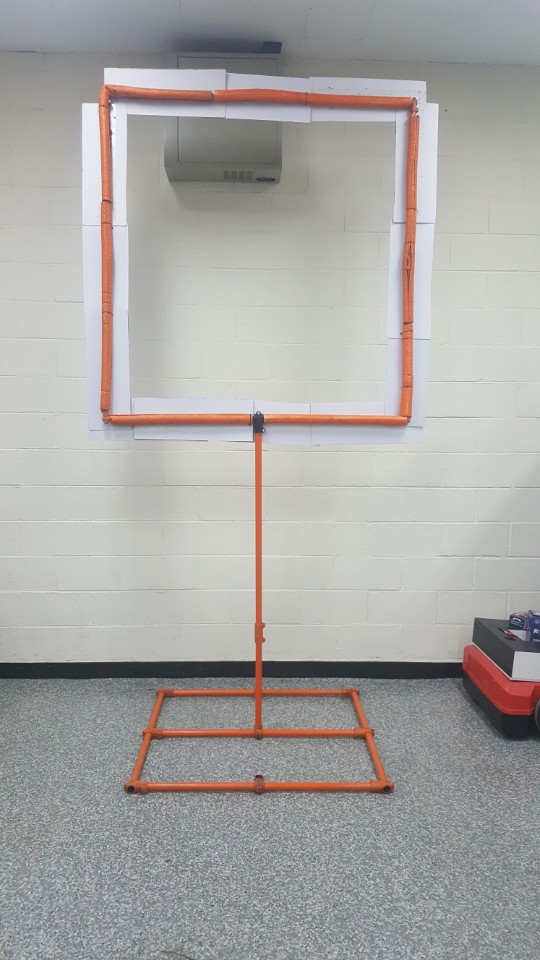
\includegraphics[height=5cm]{fig/closed_real}
	\end{minipage}\hfill
	\begin{minipage}{0.45\linewidth}
		\centering
		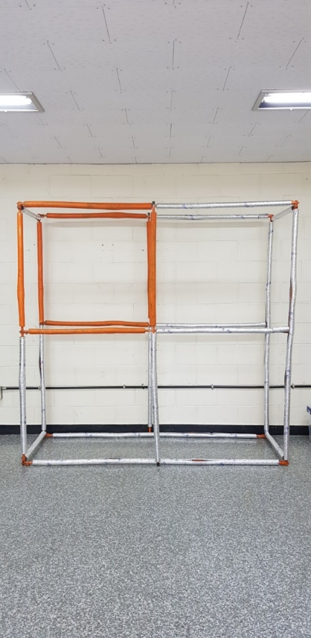
\includegraphics[height=5cm]{fig/jungle_real}
	\end{minipage}
	\caption{Example Images of the Empty Wire Frame Objects investigated in this thesis. }
	\label{fig:gates}
\end{figure}

A drawback of Deep Learning based vision systems is their need for vast amounts of annotated examples, which is not always available. Racing gates for example are not an object that appears often in everyday life and therefore not many example images exist. To this end no publicly available dataset can be used to train a Computer Vision system for \ac{EWFO}. Since a large part of the object consists of background, it is particularly crucial that the training set covers a large variety of backgrounds. Otherwise, it is likely that a model uses the background for prediction and only works in a particular domain (Overfitting). 

\begin{figure}[bhtp]
	\begin{minipage}{0.49\textwidth}
		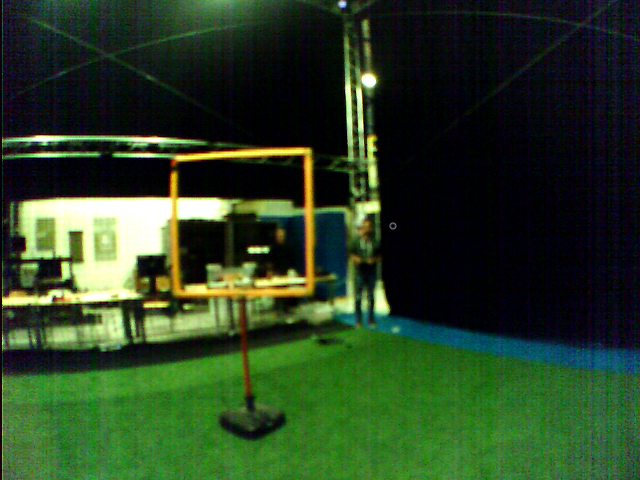
\includegraphics[width=\textwidth]{fig/real_cyberzoo2}
	\end{minipage}
	\begin{minipage}{0.49\textwidth}
		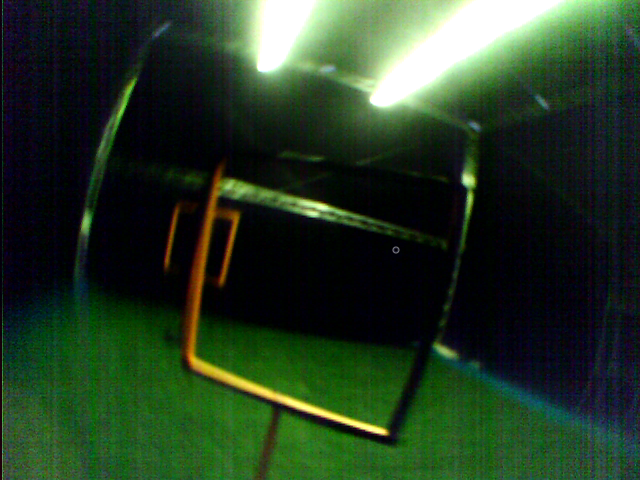
\includegraphics[width=\textwidth]{fig/real_cyberzoo1}
	\end{minipage}
	\label{fig:examples}
	\caption{Example of the \text{Cyberzoo} dataset. On the left an image while the \ac{MAV} is hovering, on the right an image during a turn manoevre.}
\end{figure}

In \Cref{fig:examples} example images of the target domain of this work are displayed. The images are taken during a test flight at a test environment. The left image shows an example when the \ac{MAV} is hovering and thus is in a very stable position. The object in this case is clearly visible as a single orange square. In contrast the right image shows a close up example during a turn manoeuvre. Here it can be seen how the used wide angle lens causes distortion and thus the lines appear as circular shape. Furthermore, large parts of the image including the horizontal bars of the object in the back appear blurred due to the circular velocity of the \ac{MAV}. In addition, the light conditions of the environment significantly influence the object appearance.

While it is possible to remove lens and sensor effects in post-processing, this can lead to information loss and requires on-board resources. Instead it is computationally more efficient to perform the detection on the raw image data. However, sensor effects have been shown to significantly influence the performance of neural networks \cite{Andreopoulos2012,Dodge2016a}. Furthermore, they can lead to varying object appearance on different \acp{MAV}. This further complicates the collection of annotated examples.
 
Another option is the artificial generation of data. By synthetically generating samples with corresponding labels, the theoretical amount of training data is infinite. Moreover, the generation allows to incorporate domain specific properties such as motion blur or image distortion. Hence, data generation is particularly useful for the detection of \acp{MAV} on \acp{EWFO} where a large variety of backgrounds is required while samples are difficult to obtain. Finally, as \ac{MAV} are brittle vehicles and mistakes in development can lead to damage on hardware, engineers and researchers often use simulators to evaluate their systems before transferring them to the real work. Thus the basic infrastructure required to generate data is often already available. 

Yet introduces the generation of data its own challenges. First and foremost because the generation process in itself is based on model assumptions. If these do not sufficiently capture the real world, a model trained in such an environment might be heavily biased and perform poorly in the real world. Secondly, because the generation of visual data is computationally intense. Despite advances in Computer Graphics can virtual environments not yet fully capture the real world. Hence, this work investigates the use of data generation in order to detect \acp{EWFO} on \acp{MAV}.

Without an accurate detection of the racing gate, the \ac{MAV} is not able to determine its current position and thus to calculate its flying trajectory. On the other hand, with an algorithm that requires less computational resources a lighter \ac{MAV} can be built. This allows faster and more aggressive trajectories as well as longer battery life. Moreover, the vision system is part of a greater state estimation and control system which also includes further sensor measurements. Depending on the remaining part of the system, faster and less accurate detections can be more useful than slow but accurate detections. Hence, the trade-off between accuracy and inference speed is of particular interest for this application and is addressed in this work.

\section{Research Question}

This section summarizes the research question addressed in this thesis. Furthermore it describes how the question is split in multiple subquestions that are addressed in the individual chapters.

	\textbf{How can \acp{CNN} detect \ac{EWFO} on \acp{MAV}, using synthetic training data?}


\begin{enumerate}
	\item[\textbf{RQ1}]How can data be generated to train a detection model for \ac{EWFO} detection on a \acp{MAV}?
	\item[\textbf{RQ2}]What kind of architecture is suitable to detect \acp{EWFO}?
	\item[\textbf{RQ3}]What are the trade-offs in detection performance and inference time when a detection model for \acp{EWFO} is deployed on a \ac{MAV}?
	\item[\textbf{RQ4}]Can the gained insights be used to build a lightweight and robust detection model for racing gates in the \ac{IROS} Autonomous Drone Race?
\end{enumerate}

\section{Results/Contributions}

\todo{Put some results at the end.}

\section{Outline}

\todo{Refactor contributions once done}
\begin{figure}[hbtp]
	\centering
	\includegraphics[width=\textwidth]{fig/outline}
	\caption{Thesis Outline}
	\label{fig:outline}
\end{figure}


The thesis is structured as displayed in \Cref{fig:outline}. \Cref{sec:metrics} describes the metrics and systems used for evaluation. \Cref{sec:training}, \Cref{sec:object_detection}, \Cref{sec:tradeoff} and \Cref{sec:method} address the individual research questions. Each chapter contains an introduction to the topic, the methodology used in this thesis and experiments that have been carried out. \Cref{sec:training} describes methods to generate synthetic data for machine learning. It concludes with the datasets used for the remaining parts of this thesis.  \Cref{sec:object_detection} describes object detection and evaluates current methods in the application for \acp{EWFO}. \Cref{sec:tradeoff} illustrates and evaluates measures to reduce computations and optimize an object detection system for a particular hardware. It investigates the trade-off between detection performance and inference time. \Cref{sec:method} describes how the gained insights are used to develop a detector for racing gates at the \ac{IROS} 2018 Autonomous Drone Race. It also compares the current method to a traditional image processing method in terms of speed and detection performance. \Cref{sec:disc} discusses the overall results and formulates a conclusion.




\chapter{Evaluation Metrics}
\label{sec:evaluation}

\todo{describe metrics and hardware}
\chapter{Transfer Learning}
\label{sec:training}

Supervised machine learning relies on the assumption that a hypothesis $h$ can be learned from a limited set of samples $X$ with their corresponding set of labels $Y$. The goal is to learn $h$ from a source set $D_s = \{X_{s},Y_{s}\}$ such that it can be applied on a target set of unknown examples $D_t = \{X_{t}\}$ to obtain the corresponding labels:

$$
h(X_t)\rightarrow Y_t
$$ 

Whether $h$ is performing well, can evaluated by splitting the labeled set of $D_s$ in a training set $D_{train}$ and test set $D_{test}$. $h$ is learned using the full information of $D_{train}$ and applied on the $D_{test}$. By evaluating a performance metric $m_A$ on $D_{train}$ information about the representation strength of $h$ can be inferred. The performance metric $m$ on $D_{test}$ gives an estimate of the performance of $h$ on $D_t$. Comparing $m_A$ and $m$ allows to evaluate whether model and dataset are suitable for the task.
			
This basic supervised machine learning setting relies on the assumption that $D_s$ follows the same i.i.d distribution as $D_t$. However, this can not be assumed for the application of this thesis. As most of the data is artificially created it will share properties with the real data but only to the extent that they can be modeled during creation. For example a graphic engine can not fully capture visual properties of all materials and light sources. Furthermore, is this model developed for application in locations with unknown light conditions and object variances that can be significantly different to the ones used at training time. When the source domain $S$ only shares a subset of properties with the target domain $T$ this is also referred to as a domain shift scenario. 


Learning models in such an environment is concerned by the field of Transfer Learning. The goal is to find a concept $h$ that performs best in the target domain $T$. Similar to $m_A$ and $m$ the performance $m_s$ in $S$ and the performance $m_t$ in $T$ can be used to evaluate whether a suitable model/dataset has been chosen/is available.

The task of learning from synthetic data can be summarized in:

$$
\text{arg}\max\limits_{h,S} m_t
$$

The goal is to create source domain $D_s$ and find a concept $h$ that maximizes its performance in the target domain $m_t$. This formulation yields two levels at which the domain shift problem can be addressed: (1) focusing on generating data or (2) focusing on finding a hypothesis that maximizes the performance.

In this thesis two types of domain shifts are considered: (1) A semi-supervised domain shift between synthetic data and real images. This means $D_s$ is available in large quantity, namely it is generated by a graphical engine. For $D_t$ a considerably smaller amount of labels is available \todo{describe real datasets}. 
(2) An unsupervised domain shift when environment conditions at test time can be significantly different to the ones at training time. In this case information about $D_t$ is only available as graphical models of the object of interest and several images of the domain. \todo{double check is this really an unsupervised domain shift since we dont even know X}

The conducted research is limited to \ac{CNN}-based object detection as they are investigated in this thesis. The chapter focuses on domain adaption while the exact model is described in \autoref{sec:object_detection}.

The relevant question to be investigated in this chapter is the following:

\begin{center}
	\textbf{How can data be generated to train a model for wire frame object detection?}
	\textbf{How can the model be made robust against domain shifts?}
\end{center}

The first question will be answered by choosing a state of the art method for object detection and training it with varying properties in $D_s$. By evaluating $m_s$ on synthetic data and $m_t$ on real images the influence of these properties will be measured.  

The second question will be answered by simulating a domain with synthetic data. That is the model will be trained in a room with significant different environment properties $D_s$ from the room it is tested in $D_t$.

The remaining parts of this chapter are structured as follows: \autoref{sec:training:related} discusses relevant related work. Based on the gained insights \autoref{sec:training:hypothesis} formulates several hypotheses to be investigated. \autoref{sec:training:experiments} outlines the experiments conducted to evaluate the formulated hypotheses. \autoref{sec:training:results} describes the obtained results. \autoref{sec:training:conclusion} discusses the results and answers the research question.

\section{Related Work}
\label{sec:training:related}

Domain shifts have been intensively studied in Machine Learning. 

A recent work \cite{Chen2018c} concerns the domain shift for object detection with deep neural networks. Based on the $\mathcal{H}$-Divergence \cite{Ben-David2010} domain classifiers are included in the network on the higher order feature activations. By incorporating the classifier in the training process and using a gradient reverse layer \todoref{gradient reverse} the feature activations are forced to be more similar. This enables to perform feature alignment in and end-to-end training process.

\cite{Xu2017} incorporate the domain adaptation by adversarial training. In a first step the network is trained using samples for the target and source domain. The obtained feature extractor is used to train a domain classifier. Finally the feature extractor is updated by inverting the domain classifier loss function and thus aligning the feature extractors.

\cite{Inoue} use variational auto encoders to create synthetic images.

\cite{Rozantsev} estimate parameters from real images to render synthetic images.

\cite{Peng2017} includes task-irrelevant samples and a source classifier to make the final network robust (?). Called zero-shot domain adaptation as no samples of the target domain are required.

\cite{Liu2018a}

\cite{Peng} use 3D CAD-models to augment the data during training.

Incorporating Camera Effects:
\cite{Carlson2018}
\begin{itemize}
	\item heaps of references in how camera properties influence object detectors
	\item introduces image augmentation pipeline based on physical model: chromatic aberration, blur, exposure, noise and color shift
	\item input parameters are modelled by hand, then randomly selected within "realistic" range
	\item no lense distortion
	\item method seem to benefit for small objects and when oversaturation applies due to camera effects
\end{itemize}


\cite{Vass}

Image Augmentation
\cite{Bai2017},

\ac{DR} was initially introduced by \cite{Tobin2017} for object localization. In contrast to domain adaptation approaches the method does not try to model the domain shift. Instead large variability in the source domain shall enable the model to learn a robust representation that is domain agnostic. \cite{Tremblay2018a} extends the approach to object detection.

The data is generated by a graphical engine. The following properties of the scene and the object are varied \cite{Tremblay2018a}:

\begin{enumerate}
	\item number, type and texture of objects of interest
	\item number, types, colours, scales of irrelevant objects (distractors)
	\item background image
	\item camera pose
	\item light sources
	\item visibility of ground plane
\end{enumerate}

An advantage of \ac{DR} is its ease of implementation and use, no assumptions about the target distribution have to be made neither are samples or labels of the target domain required. However, the method can fail to capture important patterns if the randomization is too strong. For example the movement pattern of a \ac{MAV} is ignored when placing the camera randomly.
 
\section{Approach}
\label{sec:training:hypothesis}

While a lot of approaches discussed in \autoref{sec:training:related} aim to learn a general representation that works across domains, other approaches try to incorporate more target domain knowledge to improve performance. 

It is to expected that there is a trade-off between generalization and specialization. For example placing the gates align only in positions that are physically possible allows the model to pick up context cues and thus should simplify the learning problem. Although, such a model will maybe not be able to detect objects at random positions, it is likely to never see them in the real world. 

On the other hand if the light conditions are limited to a certain room the model is likely to perform well there but will fail as soon as applied in another room. Therefore, what patterns the model is variant and invariant to is a design choice depending on the application.

The more general the model has to be, the poorer it might perform in a specific domain or the more complex it has to be. On the other hand a much simpler model can be used if particular properties are chosen to be embedded in the training domain. \todo{mention bias variance trade off here?}

This leads to the formulation of two hypothesis to be investigated:

\begin{enumerate}
	\item[H1] The more similar the properties between $D_s$ and $D_t$ the higher $m_t$ of a fixed model.
	\item[H2] The less similar the properties between $D_s$ and $D_t$ the more complex a model has to be to keep $m_t$.
\end{enumerate}



\section{Experiments}
\label{sec:training:experiments}

The experiments conducted

Initially those domain properties are investigated that can be controlled when creating the training data. The domain shift between synthethi
\begin{enumerate}
	\item \textbf{Background.} 
	
	Background refers to how the object is embedded in the environment. For example if synthetic objects are placed on random backgrounds this will not necessarily represent the background in the real world.
	
	The property can be influenced when creating the object scene: (1) The objects can be placed on randomly selected images, (2) The background can be chosen according to some properties, e.g. their similarity to the target domain. (3) A full scene can be rendered when creating data.
	
	\item \textbf{Object Placement.} 
	
	Object placement refers to the object's location in the scene. For example one would not expect an apple placed at the ceiling of a room.
	
	This property can be controlled when placing the images in background: (1) The objects can be placed at a random location on the background. (2) The objects can be placed similarly as in the target domain.
	
	\item \textbf{Illumination.} 
	
	Light conditions can influence the object appearance and its background.
	
	This property can be controlled by the graphic engine: (1) A sun-like light source can be used that spreads equally across the scene. (2) More particular light sources can be used e.g. for simulation artificial indoor light.
	
	
	\item \textbf{Camera Placement.} 
	
	Camera placement refers to the view point of the camera. For example on an \ac{MAV} the view point is limited within a range where it is still possible to fly. Randomly placing the camera does not capture such patterns.
	
	This property can be controlled when synthesizing data: (1) The camera can be placed randomly in the scene, as long as the object is still visible. (2) The camera can be placed based on the expectations in the target domain. (3) The camera can be placed following a physical model of a drone.
	
	\item \textbf{Camera Properties.} Camera properties refers to the intrinsic camera parameters. For example lens distortion can significantly influence the appearance of an object.
	
	(1) Random properties (2) Camera model, distortion model.
	
	\item \textbf{Noise.} Noise can be created by different sources. For example is noise introduced by the sensor, but also by camera motion.
	(1) Gray/Colour noise (2) Motion blur
	
\end{enumerate}

\todo{Prepare a synthetic dataset of several rooms}
\todo{Prepare a real dataset of at least two rooms}

\todo{Mesaure similarity between generated set and real set: label distribution (h,w, location, angles), domain(?), h divergence}

\todo{Quantify each property. Make a plot performance vs more effects}



\section{Results}
\label{sec:training:results}

\section{Conclusion}
\label{sec:training:conclusion}

%\section{Summaries}
%\subsection{Modeling Camera Effects to Improve Deep Vision for Real and Synthetic Data\cite{Carlson2018}}
%

	\chapter{Detecting \ac{EWFO} in Simulation}
	\label{sec:object_detection}
	
	\subsection{Reducing Inference Time}
	
	A major drawback of \acp{CNN} is their huge computational requirements. For example a state-of-the-art Computer Vision model \cite{He2015} requires 11.3 billion floating point operations \cite{Tschannen2017}. For a device with computational limitations like an \ac{MAV} this is prohibitive. Furthermore, a perception system on a \ac{MAV} usually contains of multiple subsystems. Hence, a fast reaction time can be more important than an accurate detection/outbalanced by the filter etc.
	
	This
	
	The research question of this chapter is stated as:
	
	\begin{center}
		\textbf{What are the trade-off's between detection performance $m$ and inference time $t$ when a detection model is integrated on a embedded computing platform?}
	\end{center}
	
	The question is answered on a theoretical level by using the total number of \ac{Multiply-Adds} $N_O$ as an indication for the inference time of the model. However, as also stated by \todoref{others} $N_O$ is not necessarily directly related to $t$. On a computing platform $t$ also depends on:
	
	\begin{enumerate}
		\item whether several operations can be executed in parallel,
		\item the memory usage of the operations, the kind of operation e.g. floating point or integer
		\item the particular low level implementation of the model
	\end{enumerate} 
	
	Hence, in addition to $N_0$ also the actual inference time of the model is measured on a particular computing platform.
	
	The chosen hardware is a Jevois Smart Camera \todoref{jevois}. The platform is developed for vision applications and provides a 4 Core CPU, as well as a small GPU \todo{more info}. That's why it is perfectly suitable for integrating in lightweight \acp{MAV} or other robotic applications.
	
	The rest of the chapter is organized as follows: \autoref{sec:tradeoff:related} discusses relevant related work. Based on the gained insights \autoref{sec:tradeoff:hypothesis} formulates several hypotheses to be investigated. \autoref{sec:tradeoff:experiments} outlines the experiments conducted to evaluate the formulated hypotheses. \autoref{sec:tradeoff:results} describes the obtained results. \autoref{sec:tradeoff:conclusion} discusses the results and answers the research question.
	
\chapter{Discussion}

In this work we investigated a learning based approach for the detection of \acp{EWFO} on \acp{MAV}. The research was motivated by several drawbacks of the manual crafted detection method SnakeGate. The aim was to investigate whether a learning based Object Detector is more robust against, occlusion, out of view and changes in illumination. Our results show how the deep learning based detector outperforms SnakeGate especially in the cases of occlusion and out of view. The deep learning based detector can detect objects even when only 30\% of the object is visible or when backlight leads to strong changes in colour appearance.

Yet the deep learning based detector introduces its own drawbacks. For example the bounding boxes are generally less accurate than of SnakeGate. We assume that the reason is the general structure of \ac{Yolo}. \acp{CNN} collect "shallow" low level image features and combine them to a more deep representation of the image. Pooling layers reduce the spatial resolution to keep the number of computations tracktable, however thereby also local information about the features gets lost. In the final layers information is present which features are present in that part of the image, however it is not clear where they come from. 

This not only leads loss in localization accuracy but also to lack of transparency. In some scenarios a clearly visible gate is not detected by the \acp{CNN}. In this case it is hard to find out what part of the input image led to this wrong decision. In contrast for a simple algorithm such as  \textit{SnakeGate} it is clear at all times which input information led to a decision.

 Future work should address how to reflect back from the deep representation to the low level features.

A main argument for deep learning detectors is the fact that they can be trained on any kind of object and thus make feature engineering unnecessary. Furthermore, the learned representation are often much better than the features crafted manually. A drawback is the computational requirements of \acp{CNN}. For this work no training data was available and the computational requirements were limited. By implementing a data generation pipeline and refining the architecture we could show how the deep learning based method outperforms the manually crafted one. However, this process was a vast amount of work and yet we have a severe drop in peformance between the simulated and the real data. Hence, we have to wonder whether it would have not been more fruitful to invest time in feature engineering based on real data. It is questionable whether this is method would still perform better than the deep learning method. And yes for a new object it would required to be changed. But it would lead to a more transparent detector.
\todo{deep detector can be better extended but we loose track of whats going on, deep learning makes sense with the appropriate hardware and the appropriate data}
\chapter{Conclusion \& Future Work}
\label{sec:conclusion}
This work investigated the detection of \acp{EWFO} on \ac{MAV} using a \ac{CNN}. In this section a final discussion is given and a conclusion is derived. Furthermore, the research questions are answered and possible future work is discussed.


The research was motivated by the promising results of Deep Learning based Object Detectors and several drawbacks of manually crafted algorithms for the detection of racing gates in \ac{MAV} races. As the manually tuned features prove to be sensitive to light changes as well as to object occlusion, the aim was to investigate a more robust method. 

As no real training data were available, images and corresponding object labels were created with a simulator in order to train the \acp{CNN} based Object Detector \textit{YoloV3}. We hypothesized that due to the simple shape of \acp{EWFO} a small network should be able to learn the detection task. This led to the two research questions of this work which are now answered based on the conducted experiments.

\begin{enumerate}
	\item[\textbf{RQ1}]How can data be generated to train an object detector for \ac{EWFO} detection on a \acp{MAV}?
	
	It could be seen how the detector is sensitive to overfit to environmental conditions present in the training set. When testing a detector in a different simulated environment than the training set, the performance deteriorates between 30\% and 70\%. It was further investigated how to make the detector more invariant against such environmental changes. The results show how the variance in background is less important than the creation of realistic light conditions in the training set.
	
	When a wide range of view angles is introduced in training and test sets, the performance drops particularly for larger objects. It seems the detector has difficulties learning the detection from many angles. Better performance can be achieved by reducing the number of view angles in the training set. As this raised the question of how to create realistic view points, we proposed to simulate a flight through a race court. This way the created samples resemble the real world better. Even on unseen race courts, the detector achieves a precision of 70\% compared to the 20\% achieved by the network trained without simulating a flight. 
	
	Both methods of view point generation \todo{here you mention "both methods", but you didn't mention the 2 before in the conclusion} lack of control about the actual samples present in the training set. It is hard to think about all the view points that are required to train the network for a \acp{MAV} race. However, more control about the view points could give more insights about how the detector performs with different view angles in training and test set. Hence, future work could extend the data generation tool with more control about the view points and to conduct further experiments in that respect.
		
	In order to transfer the detector to the real world, it was found that image augmentation is crucial. Particularly modelling distortion improved the results on the real data. Yet there remains a gap between the results obtained in simulation and on real data. It cannot fully be resolved whether this is because of the complexity of the real data, or whether there are certain properties missing in the data generation process. Future work could address this issue by including real data in the training process. If this improves the results significantly, the problem is likely because of a reality gap. Otherwise, there might be a more fundamental problem in the chosen detector/complexity of the test set.
	
	In summary, we propose to fully synthesize environments when creating training data for the detection of \acp{EWFO} on \acp{MAV}. Furthermore, the precision can be improved by training the detector based on view angles it will see in the real world, possibly by simulating the flight behaviour. In order to transfer the detector to the real world, we recommend to use image augmentation. Particularly augmenting the images by modelling lens distortion improves the performance on the investigated dataset.

	\item[\textbf{RQ2}]How can \acp{EWFO} be detected using a \acp{CNN} on a \acp{MAV}?
	
	The \textit{YoloV3} can be adapted to the detection of \acp{EWFO}. The experiments showed how the detector can be confused by structures that are present within the empty part of the object. This was resolved by providing samples from different backgrounds and light conditions. We hypothesized that many backgrounds are required to achieve background invariance. However, the experiments showed that a small number of different environments is already enough to make the detector more robust against such confusion.
		
	A general drop of recall was observed for closer objects. It can be assumed that this is because it is more likely that object parts are out of view when the object comes closer. For the detection of racing gates on \acp{MAV} this result can be taken into account in later stages of the control loop. For example by using a dedicated detector for closer gates and combining the information. \todo{and by including a confidence value of the predictions into the control loop?} For the general detection of \acp{EWFO}, this result is interesting. Despite being clearly visible for a human, the detector struggles in some examples. Further experiments could include investigating how the performance changes when the detector is trained without any context such as the object pole.
	
	As \acp{EWFO} consist of relatively simple features, we hypothesized that a small network should be able to learn the task. The results showed that a shallow network of 9 layers performs equally well than a network with 15 layers. However, further reducing depth gradually reduces performance from 51\% to 35\%. When reducing the width of a network with 9 layers it can be seen how the performance slowly deteriorates from 51\% at its original size to 38\% to a fraction $\frac{1}{16}$ of its original size. 
	Hence, we conclude that a minimum of 9 layers is required if detection performance is the most important metric.
	
	For the detection of \acp{EWFO} on \acp{MAV} computational resources are more important. Our results show that a network with only one filter in the first layer can still achieve 38\% average precision. Hence, by reducing the network size to 0.4\% of its original size the performance drops only by 13\% average precision.\todo{do you have numbers to indicate the speed increase in this case?}
	
	The reduction of network size was taken out by retraining the network with a thinner architecture. An alternative way of reducing the network size is to apply \textit{Knowledge Distillation} (\Cref{sec:background}). This method showed promising results on deeper network. In future work it could similarly be applied for the detection of \acp{EWFO}.
	
	The trained detector was deployed on an example \ac{MAV}. The results show how by reducing the resolution the inference time can be increased significantly. However, the costs in terms of average precision are large. Instead we propose to remove pooling layers and to use layers with larger strides. This parameter allows to trade-off between average precision and inference speed. \todo{do you have numbers showing that? or references?}
	
	An alternative way to increase the network speed is \textit{weight quantization} (\Cref{sec:background}). As the target system of this work supports floating point multiplications, we did not further consider it. However, with an adequate low level implementation this could still lead to further speed up and should be investigated in future work.
	
	In a nutshell, it could be seen that a small network is able to learn the task. The inference time of the detector can be further increased without loosing too much performance. Finally, replacing pooling layers by convolutions with larger strides allows to trade-off between detection performance and inference speed.
		
\end{enumerate}

\todo{maybe add a short summary of your contributions: you have a trained CNN for efficient detection on MAV, you have recommendations on dataset construction and on CNN optimization, you can infer from the detailed analysis of the experiments results (all the bins you made) the limitations of your detector but that is not really an "issue" because you can use this info in the control loop}

Based on the experiments a detector could be developed and compared against the baseline. The experiments showed an improvement of performance compared to \textit{SnakeGate} of up to 16\% average precision, leading to a total of 32 \% $ap_{60}$. This improvement is mainly obtained in cases of difficult light conditions or occlusion. Hence, it can be concluded that indeed the \acp{CNN} can work better in such situations.

A network of similar complexity achieves 41\% $ap_{60}$ on a simulated data set which contains more objects and more difficult view angles. Therefore it can be seen that the potential of the learning based detector is much higher. Yet transferring the detector to the real world proves to be difficult, despite the relatively simple features of \acp{EWFO}. In some cases the object is clearly visible but not detected by the \acp{CNN}. These results show the general drawback of Deep Learning based approaches. It is not transparent why the objects are not detected and what exactly was learned by the network.

A frequent argument for Deep Learning is that it does not require cumbersome Feature Engineering. In this work, this step was technically replaced by Data Engineering and yet the remaining reality gap is high and some results are hard to understand. We have to ask ourselves if the lack of transparency, the amount of required data as well as the computational requirements are really worth the results gained in detection performance. \todo{haha, that's a pretty negative formulation.....}

Nevertheless, this work serves as a baseline for future work. The initial experiments show how a small amount of environments is already enough to make the detector relatively invariant against background. These results should apply similarly to the real world. Hence, it is not too much work to create a real world training set, and the data could be augmented with the data created in this work.

Furthermore, the experiments show trade-offs in speed and detection performance. The results can be used to design a detector for \acp{EWFO} based on available hardware and project requirements.





%\section{Method}
\label{sec:method}


\input{chapters/03_method/model}
\chapter{Transfer Learning}
\label{sec:training}

Supervised machine learning relies on the assumption that a hypothesis $h$ can be learned from a limited set of samples $X$ with their corresponding set of labels $Y$. The goal is to learn $h$ from a source set $D_s = \{X_{s},Y_{s}\}$ such that it can be applied on a target set of unknown examples $D_t = \{X_{t}\}$ to obtain the corresponding labels:

$$
h(X_t)\rightarrow Y_t
$$ 

Whether $h$ is performing well, can evaluated by splitting the labeled set of $D_s$ in a training set $D_{train}$ and test set $D_{test}$. $h$ is learned using the full information of $D_{train}$ and applied on the $D_{test}$. By evaluating a performance metric $m_A$ on $D_{train}$ information about the representation strength of $h$ can be inferred. The performance metric $m$ on $D_{test}$ gives an estimate of the performance of $h$ on $D_t$. Comparing $m_A$ and $m$ allows to evaluate whether model and dataset are suitable for the task.
			
This basic supervised machine learning setting relies on the assumption that $D_s$ follows the same i.i.d distribution as $D_t$. However, this can not be assumed for the application of this thesis. As most of the data is artificially created it will share properties with the real data but only to the extent that they can be modeled during creation. For example a graphic engine can not fully capture visual properties of all materials and light sources. Furthermore, is this model developed for application in locations with unknown light conditions and object variances that can be significantly different to the ones used at training time. When the source domain $S$ only shares a subset of properties with the target domain $T$ this is also referred to as a domain shift scenario. 


Learning models in such an environment is concerned by the field of Transfer Learning. The goal is to find a concept $h$ that performs best in the target domain $T$. Similar to $m_A$ and $m$ the performance $m_s$ in $S$ and the performance $m_t$ in $T$ can be used to evaluate whether a suitable model/dataset has been chosen/is available.

The task of learning from synthetic data can be summarized in:

$$
\text{arg}\max\limits_{h,S} m_t
$$

The goal is to create source domain $D_s$ and find a concept $h$ that maximizes its performance in the target domain $m_t$. This formulation yields two levels at which the domain shift problem can be addressed: (1) focusing on generating data or (2) focusing on finding a hypothesis that maximizes the performance.

In this thesis two types of domain shifts are considered: (1) A semi-supervised domain shift between synthetic data and real images. This means $D_s$ is available in large quantity, namely it is generated by a graphical engine. For $D_t$ a considerably smaller amount of labels is available \todo{describe real datasets}. 
(2) An unsupervised domain shift when environment conditions at test time can be significantly different to the ones at training time. In this case information about $D_t$ is only available as graphical models of the object of interest and several images of the domain. \todo{double check is this really an unsupervised domain shift since we dont even know X}

The conducted research is limited to \ac{CNN}-based object detection as they are investigated in this thesis. The chapter focuses on domain adaption while the exact model is described in \autoref{sec:object_detection}.

The relevant question to be investigated in this chapter is the following:

\begin{center}
	\textbf{How can data be generated to train a model for wire frame object detection?}
	\textbf{How can the model be made robust against domain shifts?}
\end{center}

The first question will be answered by choosing a state of the art method for object detection and training it with varying properties in $D_s$. By evaluating $m_s$ on synthetic data and $m_t$ on real images the influence of these properties will be measured.  

The second question will be answered by simulating a domain with synthetic data. That is the model will be trained in a room with significant different environment properties $D_s$ from the room it is tested in $D_t$.

The remaining parts of this chapter are structured as follows: \autoref{sec:training:related} discusses relevant related work. Based on the gained insights \autoref{sec:training:hypothesis} formulates several hypotheses to be investigated. \autoref{sec:training:experiments} outlines the experiments conducted to evaluate the formulated hypotheses. \autoref{sec:training:results} describes the obtained results. \autoref{sec:training:conclusion} discusses the results and answers the research question.

\section{Related Work}
\label{sec:training:related}

Domain shifts have been intensively studied in Machine Learning. 

A recent work \cite{Chen2018c} concerns the domain shift for object detection with deep neural networks. Based on the $\mathcal{H}$-Divergence \cite{Ben-David2010} domain classifiers are included in the network on the higher order feature activations. By incorporating the classifier in the training process and using a gradient reverse layer \todoref{gradient reverse} the feature activations are forced to be more similar. This enables to perform feature alignment in and end-to-end training process.

\cite{Xu2017} incorporate the domain adaptation by adversarial training. In a first step the network is trained using samples for the target and source domain. The obtained feature extractor is used to train a domain classifier. Finally the feature extractor is updated by inverting the domain classifier loss function and thus aligning the feature extractors.

\cite{Inoue} use variational auto encoders to create synthetic images.

\cite{Rozantsev} estimate parameters from real images to render synthetic images.

\cite{Peng2017} includes task-irrelevant samples and a source classifier to make the final network robust (?). Called zero-shot domain adaptation as no samples of the target domain are required.

\cite{Liu2018a}

\cite{Peng} use 3D CAD-models to augment the data during training.

Incorporating Camera Effects:
\cite{Carlson2018}
\begin{itemize}
	\item heaps of references in how camera properties influence object detectors
	\item introduces image augmentation pipeline based on physical model: chromatic aberration, blur, exposure, noise and color shift
	\item input parameters are modelled by hand, then randomly selected within "realistic" range
	\item no lense distortion
	\item method seem to benefit for small objects and when oversaturation applies due to camera effects
\end{itemize}


\cite{Vass}

Image Augmentation
\cite{Bai2017},

\ac{DR} was initially introduced by \cite{Tobin2017} for object localization. In contrast to domain adaptation approaches the method does not try to model the domain shift. Instead large variability in the source domain shall enable the model to learn a robust representation that is domain agnostic. \cite{Tremblay2018a} extends the approach to object detection.

The data is generated by a graphical engine. The following properties of the scene and the object are varied \cite{Tremblay2018a}:

\begin{enumerate}
	\item number, type and texture of objects of interest
	\item number, types, colours, scales of irrelevant objects (distractors)
	\item background image
	\item camera pose
	\item light sources
	\item visibility of ground plane
\end{enumerate}

An advantage of \ac{DR} is its ease of implementation and use, no assumptions about the target distribution have to be made neither are samples or labels of the target domain required. However, the method can fail to capture important patterns if the randomization is too strong. For example the movement pattern of a \ac{MAV} is ignored when placing the camera randomly.
 
\section{Approach}
\label{sec:training:hypothesis}

While a lot of approaches discussed in \autoref{sec:training:related} aim to learn a general representation that works across domains, other approaches try to incorporate more target domain knowledge to improve performance. 

It is to expected that there is a trade-off between generalization and specialization. For example placing the gates align only in positions that are physically possible allows the model to pick up context cues and thus should simplify the learning problem. Although, such a model will maybe not be able to detect objects at random positions, it is likely to never see them in the real world. 

On the other hand if the light conditions are limited to a certain room the model is likely to perform well there but will fail as soon as applied in another room. Therefore, what patterns the model is variant and invariant to is a design choice depending on the application.

The more general the model has to be, the poorer it might perform in a specific domain or the more complex it has to be. On the other hand a much simpler model can be used if particular properties are chosen to be embedded in the training domain. \todo{mention bias variance trade off here?}

This leads to the formulation of two hypothesis to be investigated:

\begin{enumerate}
	\item[H1] The more similar the properties between $D_s$ and $D_t$ the higher $m_t$ of a fixed model.
	\item[H2] The less similar the properties between $D_s$ and $D_t$ the more complex a model has to be to keep $m_t$.
\end{enumerate}



\section{Experiments}
\label{sec:training:experiments}

The experiments conducted

Initially those domain properties are investigated that can be controlled when creating the training data. The domain shift between synthethi
\begin{enumerate}
	\item \textbf{Background.} 
	
	Background refers to how the object is embedded in the environment. For example if synthetic objects are placed on random backgrounds this will not necessarily represent the background in the real world.
	
	The property can be influenced when creating the object scene: (1) The objects can be placed on randomly selected images, (2) The background can be chosen according to some properties, e.g. their similarity to the target domain. (3) A full scene can be rendered when creating data.
	
	\item \textbf{Object Placement.} 
	
	Object placement refers to the object's location in the scene. For example one would not expect an apple placed at the ceiling of a room.
	
	This property can be controlled when placing the images in background: (1) The objects can be placed at a random location on the background. (2) The objects can be placed similarly as in the target domain.
	
	\item \textbf{Illumination.} 
	
	Light conditions can influence the object appearance and its background.
	
	This property can be controlled by the graphic engine: (1) A sun-like light source can be used that spreads equally across the scene. (2) More particular light sources can be used e.g. for simulation artificial indoor light.
	
	
	\item \textbf{Camera Placement.} 
	
	Camera placement refers to the view point of the camera. For example on an \ac{MAV} the view point is limited within a range where it is still possible to fly. Randomly placing the camera does not capture such patterns.
	
	This property can be controlled when synthesizing data: (1) The camera can be placed randomly in the scene, as long as the object is still visible. (2) The camera can be placed based on the expectations in the target domain. (3) The camera can be placed following a physical model of a drone.
	
	\item \textbf{Camera Properties.} Camera properties refers to the intrinsic camera parameters. For example lens distortion can significantly influence the appearance of an object.
	
	(1) Random properties (2) Camera model, distortion model.
	
	\item \textbf{Noise.} Noise can be created by different sources. For example is noise introduced by the sensor, but also by camera motion.
	(1) Gray/Colour noise (2) Motion blur
	
\end{enumerate}

\todo{Prepare a synthetic dataset of several rooms}
\todo{Prepare a real dataset of at least two rooms}

\todo{Mesaure similarity between generated set and real set: label distribution (h,w, location, angles), domain(?), h divergence}

\todo{Quantify each property. Make a plot performance vs more effects}



\section{Results}
\label{sec:training:results}

\section{Conclusion}
\label{sec:training:conclusion}

%\section{Summaries}
%\subsection{Modeling Camera Effects to Improve Deep Vision for Real and Synthetic Data\cite{Carlson2018}}
%


\chapter{Transferring it to the Real World}
\label{sec:tradeoff}


After having created a set of 2D images, the final step applies low-level image transformations. It allows to further simulate sensor effects and increase the variance in the generated data.

In literature \cite{Krizhevsky2012a,Howard2013,Redmon,Liu} the application of image augmentation is a common tool to improve the detection performance. The experiments in \cite{Carlson2018} show how the incorporation of sensor effects particularly improves the performance of models learned on fully synthesized data. In the \ac{MAV} domain sensor and lens effects have a significant influence on the obtained sample. Hence, we hypothesize that the incorporation of these effects is particularly useful for the \ac{MAV} domain.

\paragraph{Lens Distortion}

Lens distortion is a form of optical aberration which causes light to not fall in a single point but a region of space. For \acp{MAV} commonly used wide-angle lenses, this leads to barrel distortion and thus to straight lines appearing as curves in the image.

The effect is applied using the model for wide-angle lenses from \cite{Vass}. It models the removal of lens distortion as combination of radial and non-radial part, that is approximated with a second order Taylor expansion:
\todo{double check formula is (y in first line?)}
\begin{equation}
f(x,y) =
\begin{pmatrix}
x (1 + \kappa_1 x^2 + \kappa_1 (1 + \lambda_x) y^2 + \kappa_2(x^2 + y^2)^2) \\
y (1 + \kappa_1 x^2 + \kappa_1 (1 + \lambda_y) y^2 + \kappa_2(x^2 + y^2)^2)
\end{pmatrix} 
\label{eq:distortion}
\end{equation}
Where:
\begin{itemize}
	\item f yields the undistorted coordinates.
	\item $\kappa_1$ $\kappa_2$ control the radial distortion 
	\item $\lambda_x$ and $\lambda_y$ control the tangential distortion
\end{itemize}

Applying the lens distortion to an image is done using the inverse of \Cref{eq:distortion}. However, as there is no closed form solution, so the Newton-approximation.

An example with $\kappa_1 = 0.5, \kappa_2 = 0.5$ is displayed in \Cref{fig:distortion}. It can be seen how the previously straight lines appear as circular shape.

\paragraph{Chromatic Aberration.}

Chromatic Aberration is caused when different wavelengths of light do not end up in the same locations of the visual sensor. This leads to a shift in the colour channels of the image.

Similarly to \cite{Carlson2018}, chromatic aberration is applied by scaling the locations of the green channel, as well as applying translations on all channels. The model can be implemented as affine transformation of the pixel locations for each channel:

\begin{equation}
f(x_C,y_C) = \begin{pmatrix}
S & 0 & t_x \\
0 & S & t_y \\
0 & 0 & 1
\end{pmatrix} \begin{pmatrix}
x_C \\
y_C \\
1
\end{pmatrix}
\end{equation}

Where $C$ is one colour channel of the image.

An example is displayed in \Cref{fig:chromatic}. It can be seen how the red and green channel are shifted relative to each other. Thus two bars appear in the image.

\paragraph{Blur}

Motion noise is caused when light falls in different locations of the images sensor due to a fast movement of the camera. It leads to blurry images based on the sensor motion.

The phenomenon depends on camera properties as well as the motion of camera and objects. Although a full modelling of this process might benefit the learning process, it requires a complex pipeline and is computationally expensive. Therefore a strong simplification is used, namely a one-dimensional Gaussian filter:

An example for vertical blur is displayed in \Cref{fig:motionblur}. It can be seen how particularly horizontal lines appear softer.

Next to motion, sensor noise can lead to blurry images. For the blur operation a 2D Gaussian kernel is applied on the input image with:

\begin{equation}
k = \frac{1}{2\sigma_x\sigma_y\pi}e^{-\sqrt{\frac{x^2 + y^2}{2\sigma_x\sigma_y}}} 
\end{equation}
\todo{double check notation}
\paragraph{Exposure.}

Exposure is the time the sensor records light in order to create an image. Over- and Underexposure are caused when this time is too short or too long, leading to too dark or too bright images.

Following the model from \cite{Carlson2018}:

\begin{equation}
f(S) = \frac{255}{1 + e^{-A S}}
\end{equation}
where $A$ is a constant term for contrast and $S$ the exposure.
\todo{whats a}
The image can be re-exposed with:

\begin{equation}
I' = f(S+\Delta S)
\end{equation}

where $S$ is obtained from :
\begin{equation}
S = f^{-1}(I)
\end{equation}

An example for overexposure is displayed in \Cref{fig:exposure}. It can be seen how lighter areas appear particularly light, while dark areas remain dark.

\subsection{Color Variations}

\todo{describe hsv scaling}


\begin{figure}[htbp]
	\centering
	\begin{minipage}{0.33\textwidth}
		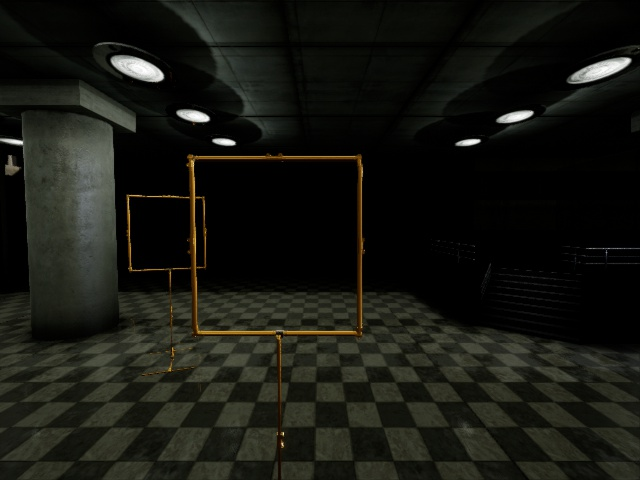
\includegraphics[width=\textwidth]{fig/gate_example}
		\caption{Original Image.}
		\label{fig:orig}
	\end{minipage}
	\begin{minipage}{0.33\textwidth}
		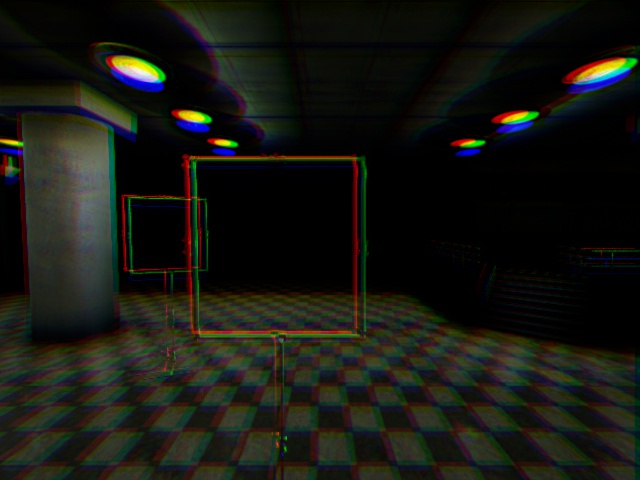
\includegraphics[width=\textwidth]{fig/gate_example_chromatic}
		\caption{Chromatic Aberration.} 		
		\label{fig:chromatic}
	\end{minipage}
	\begin{minipage}{0.33\textwidth}
		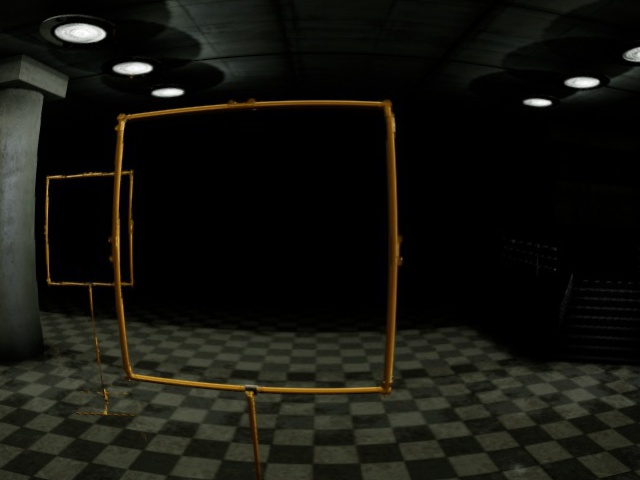
\includegraphics[width=\textwidth]{fig/gate_example_distorted}
		\caption{Lens Distortion. }		
		\label{fig:distortion}
	\end{minipage}
	
	\begin{minipage}{0.33\textwidth}
		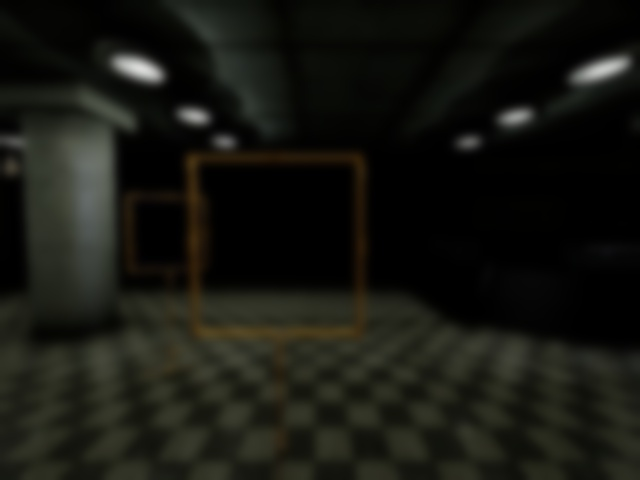
\includegraphics[width=\textwidth]{fig/gate_example_focusblur}
		\caption{Out-of-Focus blur.}
		\label{fig:focusblur}
	\end{minipage}
	\begin{minipage}{0.33\textwidth}
		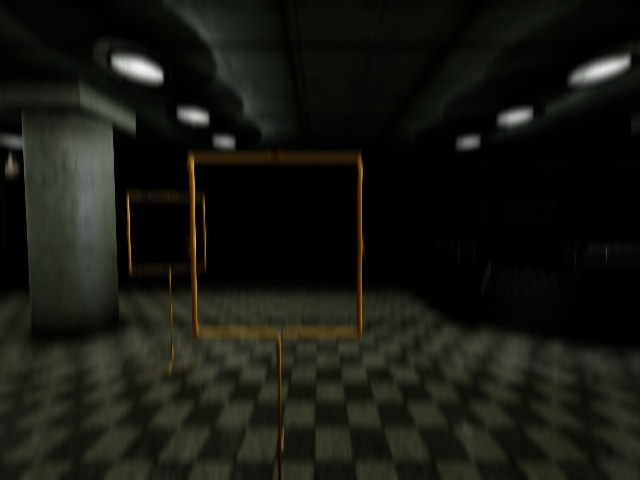
\includegraphics[width=\textwidth]{fig/gate_example_motionblur_v}
		\caption{Vertical Motion Blur.}
		\label{fig:motionblur}
	\end{minipage}
	\begin{minipage}{0.33\textwidth}
		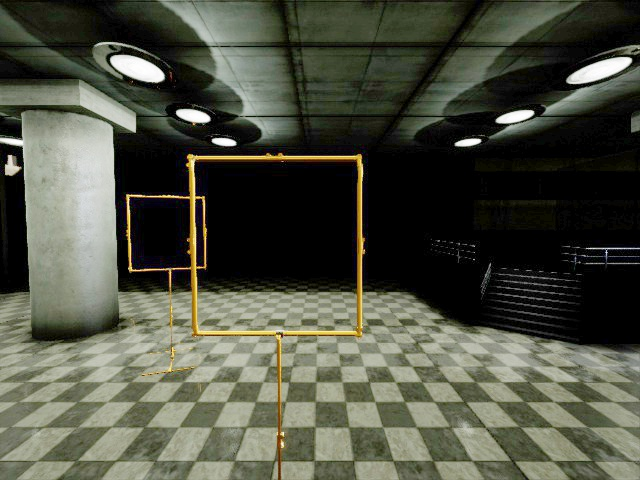
\includegraphics[width=\textwidth]{fig/gate_example_exposure}
		\caption{Exposure.}
		\label{fig:exposure}
	\end{minipage}
\end{figure}

\subsection{Hypothesis}
\label{sec:training:hypothesis}

This chapter summarizes the hypotheses formulated in the previous chapters:

\begin{enumerate}
	\item[$\mathcal{H}_1$] An object that is not empty and provides a more distinctive structure is less background dependent than an \ac{EWFO}.
	
	\item[$\mathcal{H}_2$] The incorporation of correct placement/light conditions improves the performance of a model trained to detect \acp{EWFO}.
	
	\item[$\mathcal{H}_3$] The incorporation of a camera motion model resembling the target domain improves the performance of a model trained to detect \acp{EWFO}. 
	
	\item[$\mathcal{H}_3$] Including sensor effects present in the target domain, improves the performance of a model trained to detect \acp{EWFO}. 
	
\end{enumerate}



\section{Experiments}
\label{sec:training:experiments}
In order to evaluate the formulated hypotheses several experiments are conducted. The model used is the TinyYoloV3-Architecture, further described in \Cref{sec:object_detection}. The reported metrics are described in \Cref{sec:metrics}. For all experiments mean and standard deviation of 5 runs are reported.

For the random view point generation the following parameters are used:

\begin{equation}
x = \mathcal{U}(-30,30),\quad y = \mathcal{U}(-20,20),\quad z = \mathcal{N}(-4.5,0.5)),\quad
\phi = \mathcal{U}(0,0.1\pi),\quad \theta = \mathcal{U}(0,0.1\pi),\quad \psi = \mathcal{N}(-\pi,\pi)
\label{eq:distroexp}
\end{equation}
Where $ \mathcal{U}(a,b)$ is a uniform distribution between $a,b$ and $\mathcal{N}(\mu,\sigma^2)$ is a Gaussian distribution with mean $\mu$ and variance $\sigma^2$.

The parameters are chosen experimentally aiming to resemble common view points of a person standing in the room.

\subsubsection{Experiment I}
The empty space of an \ac{EWFO} is augmented with a detailed texture. An example can be seen in \Cref{fig:cats}.
\begin{figure}
	\centering
	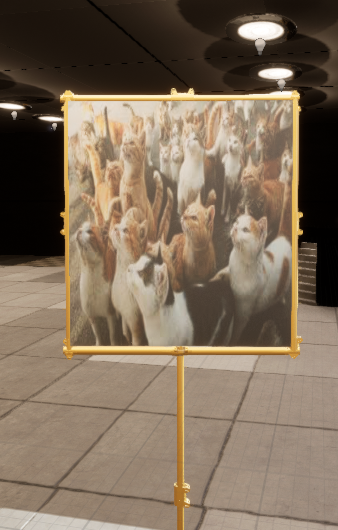
\includegraphics[height=5cm]{fig/cat}
	\caption{The \ac{EWFO} is augmented with a detailed texture.}
	\label{fig:cats}
\end{figure}

The object is placed in a scene with uniformly coloured backgrounds and a training set of 20 000 samples is created. In similar fashion a training set is created without the texture rich augmentation. The test set contains 1000 samples created in the \textit{IROS} environment by randomly placing the camera following \Cref{eq:distroexp}.




\subsubsection{Experiment II}

Several models are trained on 20 000 samples each.
\begin{itemize}
	\item[ModelU] Uniform
	\item[ModelSVE] Single Virtual Environment
	\item[ModelRB] Real Backgrounds
	\item[ModelVVE] Various Virtual Environments
	\item[ModelRBVVE] Real Backgrounds + Various Virtual Environments
\end{itemize}


\begin{table}[htbp]
	\caption{}
	\begin{tabular}{|l|l|l|l|r|r|r|l|l|l|}
		\hline
		& Validation Set &  &  & \multicolumn{1}{l|}{IROS2018} & \multicolumn{1}{l|}{} & \multicolumn{1}{l|}{} & Real Data &  &  \\ \hline
		& AP40 & AP60 & AP80 & \multicolumn{1}{l|}{AP40} & \multicolumn{1}{l|}{AP60} & \multicolumn{1}{l|}{AP80} & AP40 & AP60 & AP80 \\ \hline
		U &  &  &  & 0.05 & 0.01 & 0 &  &  &  \\ \hline
		SVE &  &  &  & 0.29 & 0.17 & 0.02 &  &  &  \\ \hline
		VVE &  &  &  & 0.61 & 0.49 & 0.17 &  &  &  \\ \hline
		RB &  &  &  & 0.42 & 0.28 & 0.04 &  &  &  \\ \hline
	\end{tabular}
	\label{tab:env}
\end{table}


\subsubsection{Experiment III}

Three models are trained: Model I using random placement, Model II using the drone motion model, Model III using a combination of both methods. In both experiments environment and light conditions as well as object locations are the same. The models are tested on two test sets: Set I created by randomly placing the camera. Set II by using the drone motion model, where a circuit is used that has not been part in the generation of the training data.


\subsubsection{Experiment IV}

In order to evaluate $\mathcal{H}_4$ the individual domain properties are measured on the target domain and incorporated in the training set.


\section{Results}
\label{sec:training:results}

\section{Discussion}
\label{sec:training:discussion}

\section{Conclusion}
\label{sec:training:conclusion}



%\chapter{Discussion}
\label{sec:disc}
\todo{answer research questions}
%% Use letters for the chapter numbers of the appendices.
\appendix

\section{Data Generation}
\label{sec:appendix:datagen}

This section describes how the ground truth labels are obtained when generating data.

\subsection{Camera Model}

\hfill \\
The camera itself is modelled with the pinhole camera model that contains six parameters:

\begin{enumerate}
	\item Focal length $f_x,f_y$
	\item Central point $c_x,c_y$
	\item Sensor skew $s_x, s_y$
\end{enumerate}

The model can be summarized in the intrinsic camera matrix $C$:
\begin{equation}
C = \begin{bmatrix}
\frac{fx}{s_x} & 0 &cx \\
0&  \frac{f_y}{s_y}&cy \\
0& 	0&	1
\end{bmatrix}
\label{eq:pinhole1}
\end{equation}

The model projects 3D coordinates $X$ to the image plane following:
\begin{equation}
X' = C X
\label{eq:pinhole2}
\end{equation}
Where $X$ are points described in homogeneous coordinates originating from the cameras position.

For data generation several tools are used. 3D Models for the \ac{TO} are taken from ... OpenGl is used to render these objects and replace the background with a particular image. The Unreal Engine and AirSim are used to render a full scene.

Within the graphic engines, the objects can be placed in 3D space. From the known object shape the surrounding bounding box can be defined in 3D coordinates. Using the pinhole camera model described in \Cref{eq:pinhole1} the corresponding 2D coordinates on the image plane can be obtained with the following:

The camera position is described by its rotation matrix $R$ and its translation vector $t$. Where $R$ is obtained from the Euler angles with:
$$
R =
$$
The 3D coordinates of the objects relative to the camera can be obtained by applying the inverse transformation $T$ of $R$ and $t$ with:
$$
t' = R \times t
$$
$$
T = R^{-1}|-t'
$$
$$
X_{Cam} = T\times X
$$
The full projection can then be expressed by the matrix multiplication:
$$
X' = C\times T\times X
$$
Where $C$ is the intrinsic camera matrix defined in \Cref{eq:pinhole1}.

\bibliography{thesis}

\end{document}

